\documentclass[11pt]{article}
\usepackage[a4paper,margin=2.3cm]{geometry}
\usepackage[T1]{fontenc}
\usepackage[utf8]{inputenc}
\usepackage{lmodern,amsmath,graphicx,xcolor,setspace,booktabs}
\usepackage[round,authoryear]{natbib}
\usepackage[colorlinks=true,linkcolor=blue!50!black,citecolor=blue!50!black,urlcolor=blue!50!black]{hyperref}
\newcommand{\degr}{\ensuremath{^\circ}}
\renewcommand{\thefigure}{S\arabic{figure}}
\renewcommand{\thetable}{S\arabic{table}}
\setstretch{1.1}
\title{Supporting Information for ``Ocean tides modulate the 26-second Gulf of Guinea microseism''}
\author{Larsen Cundric\\[6pt]
\normalsize\textit{AI-generated manuscript produced using Grok Bot}\\
\normalsize\textit{Experiment initiated and guided by Larsen Cundric}}
\date{}
\begin{document}
\maketitle

\noindent\textbf{Contents.} Texts S1--S8, Table S1, Figures S1--S11. Lags are hours after predicted M2 high water at Port Sonara (Limbe); amplitudes are M2 amplitudes in dB (half the peak-to-trough range) unless stated; brackets are 95\% intervals. Station distances are measured from a nominal source point at 4\degr N, 8\degr E. The AI-use disclosure in the main text applies to this Supporting Information as well.

\section*{Text S1. Detection and quality control}
Spectra were computed from 10,800-s windows stepped by 3600 s: a Hann-tapered periodogram zero-padded to $2^{17}$ samples, and a Welch spectrum from 3600-s segments with 50\% overlap. The line search band is 37.0--39.5 mHz; the SNR is the band maximum divided by the median of 30--34 and 42--46 mHz. The control band (30--32.5 mHz, reference 27--29.5 and 33--34.5 mHz) defines the 1\% false-alarm threshold (EDA 5.99; TAM 6.65) and 0.1\% threshold (EDA 12.15). At EDA 38,888 of 52,547 windows (74.0\%) pass quality control; 31.0\% of these are detections at 1\% false-alarm rate and 7.4\% at 0.1\%. Detection fractions over the common period are given in Table~\ref{tab:multi}. Daily detection rate at EDA correlates only weakly with ERA5 significant wave height at 3\degr N, 8\degr E ($r=0.20$). The long-term behaviour of the line at EDA is shown in Figure~\ref{fig:long}: the median period is 26.341 s [26.336, 26.347] with a trend of 15.7 ms/yr [11.7, 20.7] over 2019--2026.

\section*{Text S2. Tide reference}
The Port Sonara hourly research-quality record (UHSLC 816; 2008-06 to 2011-06) was fitted with UTide (98.9\% variance explained; M2 0.59 m, S2 0.21 m) and the fit was used to predict hourly tides for 2019--2026. In the prediction S2/M2 is 0.360 (equilibrium 0.466) and N2/M2 0.215 (equilibrium 0.191); the observed 2008--2011 S2/M2 is 0.344. The semidiurnal envelope used for the scaling tests has a mean of 0.587 m (5--95\%: 0.310--0.879 m). Fits at S\~ao Tom\'e (UHSLC 225) and Lagos (233) place M2 high water $-0.18$ h and $+0.29$ h relative to Port Sonara. Gauge L2/M2 ratios are 0.019 (Port Sonara), 0.020 (S\~ao Tom\'e) and 0.024 (Lagos), below the equilibrium 0.028. For SACV we also used the Praia gauge (UHSLC 222), whose envelope correlates with that at Port Sonara at 0.955. Over 2019--2026 the nodal cycle changes the predicted M2 amplitude by only 4\% (0.574 to 0.552 m in 2-yr windows). No contemporaneous (2019--2026) gauge data were used. Gauge coordinates (UHSLC metadata): Port Sonara 4.007\degr N, 9.127\degr E; S\~ao Tom\'e 0.348\degr N, 6.737\degr E; Lagos 6.423\degr N, 3.412\degr E; Praia 14.917\degr N, 23.5\degr W.

\section*{Text S3. Statistical methods}
\textit{Harmonic regression.} Hourly series were high-passed by subtracting a 72-h running median and regressed by least squares on cosine and sine terms for M2, S2, N2, K1, O1, Q1, M4, S1 and S3. The complex amplitude $a-ib$ gives the amplitude and lag. S2 and K1 are partly confounded with solar and thermal (S1, S2) effects and receive less weight in the interpretation; an additive solar S2 contribution is bounded at $\le0.08$ dB at EDA (Text S5).
\textit{Moving-block bootstrap.} Per-day normal-equation sums were resampled in blocks of 15 or 30 days with day-aligned random starts \citep{kunsch1989}. At EDA the variance-inflation factor relative to white-noise least squares is 2.24 (effective sample 17,336 of 38,888 hours).
\textit{Nulls.} (1) Phase-randomised surrogates with the smoothed spectrum of the series \citep{theiler1992} (500 realisations). (2) Random-start block resampling: data blocks of 15 or 30 days are moved to random positions while the tidal design matrix is held fixed, destroying the tidal phase relation but preserving within-block autocorrelation and gaps (1000 realisations). The 30-day version is the most conservative and is quoted in the main text.
\textit{Multi-station combination.} Lags were combined by inverse-variance weighting, with the weights and the mean-lag interval obtained from a joint bootstrap in which all stations share the same block draws, preserving inter-station correlation. Homogeneity was assessed with Cochran's $Q$. The hourly LMB series of EDA, TAM and SACV correlate at 0.47--0.57, and EDA--TAM high-passed log SNR at 0.48, so station results are not independent.

\section*{Text S4. Robustness of the M2 modulation}
\textit{Metric.} At EDA the M2 term is 0.548 dB at $+1.3$ h in raw fixed-band line power, 0.391 dB at $+1.7$ h in Welch SNR, 0.473 dB at $+1.6$ h in LMB, and 5.51 percentage points at $+1.6$ h in detection fraction (Figure~\ref{fig:ctrl}, \ref{fig:svs}). In detected windows alone the peak PSD has M2 0.21 dB at $+1.3$ h. The near-line backgrounds are modulated less: 20--24 s 0.13 dB ($p=0.07$), 29--34 s 0.21 dB at $+0.2$ h, 20--30 mHz 0.18 dB at $+12.2$ h. Controls: the line-free control-band SNR has a small M2 term (0.05 dB); the primary microseism (50--80 mHz) 0.07 dB ($p=0.04$) at $+10.4$ h; the secondary microseism (0.1--0.3 Hz) 0.13 dB at $+1.0$ h, as expected for a coastal station.
\textit{Sub-periods.} Leaving out any calendar year gives 0.448--0.492 dB and 1.57--1.67 h; single years give 0.284--0.602 dB and 1.33--1.85 h, with lower amplitudes in 2024--2026 (Figure~\ref{fig:loyo}).
\textit{Covariates and confounds.} Adding 72-h high-passed ERA5 log significant wave height and peak period as regressors leaves M2 at 0.473 dB at $+1.63$ h. Across envelope terciles (neap to spring) the mean ERA5 wave height (1.143, 1.154, 1.160 m) and slow line SNR are flat, while the detection rate changes only from 0.322 to 0.295.
\textit{Periodograms.} Full-band periodograms of the hourly frequency, amplitude and SNR series with surrogate levels are in Figure~\ref{fig:pgram}; cross-correlation with tidal height and phase-binned versions in Figure~\ref{fig:xcorr}.
\textit{Other constituents at EDA.} S2 0.168 dB ($+2.20$ h), N2 0.075 dB ($+2.38$ h; block $p_{30}=0.015$), S1 0.053 dB, M4 0.033 dB. With K2 added (separable from S2 over 7.4 yr), K2 is 0.046 dB [0.014, 0.100], close to the 0.054 dB expected for proportional scaling.

\section*{Text S5. Scaling with tidal range: diagnostics}
\textit{Bins and envelope model.} Five-bin results are in the main text and Figure~\ref{fig:sn}. Lags are constant across bins within errors. Over 2-yr windows $\gamma$ has a standard deviation of 0.27--0.32 at EDA and TAM and 0.44--0.50 at SACV, compared with 0.17 for EDA over 7.4 yr; if the true $\gamma$ is 0.7, a 2-yr window excludes zero only 53\% (EDA), 73\% (TAM) and 34\% (SACV) of the time (Figure~\ref{fig:cav1}). The three 2022--2024 values (EDA 0.46, TAM 0.33, SACV $-0.26$) are jointly as low as observed in 2\% of simulations with $\gamma=0.7$ and 0.3\% with $\gamma=1$ (simulations share blocks across stations). Calendar-year heterogeneity is not significant (EDA $p=0.29$, TAM $p=0.20$), and a noise-free synthetic with the real gaps returns $\gamma=1.008$ in every window. At SACV the result is not explained by the local tide (Praia envelope gives $-0.32$), local swell, or detection selection; raw line power gives $+0.44$ there, and the background bands carry positive (non-significant) envelope terms that the LMB regression subtracts. We cannot distinguish a shared noise fluctuation from a modest real change in the source's tidal sensitivity.

\textit{Errors in variables.} If the true forcing followed the S\~ao Tom\'e or Lagos tide, or S2 were mis-predicted by $\pm20\%$, the recovered $\gamma$ would be 0.93--0.94 or 0.89/1.12 instead of 1 (Figure~\ref{fig:cav2}); envelopes from the other gauges give EDA 0.69--0.77 and TAM 0.69--0.75.

\textit{Shape.} With eight bins, EDA accepts proportional scaling ($\chi^2=7.7$ for 7 dof, $p=0.36$); power-law (exponent 0.70), linear-plus-offset and saturating fits are marginally better ($\Delta$AIC $\approx$1--2) and constant amplitude is rejected ($p=0.001$). TAM bins scatter beyond their errors and no shape is decidable. A symmetric saturation $\tanh(h/0.6\,\mathrm{m})$ reproduces $\gamma=0.70$ with M4/M2 = 0.046 (observed 0.071; the tide itself 0.054); one-sided clipping or thresholds give M4/M2 = 0.14--0.32 and are excluded. Linear-in-power responses measured in dB give $\gamma=1.01$--1.80; current-driven responses give 1.02 (linear) or 1.86 ($u|u|$). A delayed response does not help ($\gamma$ peaks at 0.79 for a $+24$ h envelope lag at EDA).

\textit{Metric.} Raw line power gives $\gamma=1.01$ (EDA) and 0.32 (TAM) over the full spans, versus 0.70 and 0.68 for LMB.

\textit{Sidebands and the lunar test.} For an amplitude-modulated response the main sideband gain is $(1+\gamma)/2$ and the mirror sideband gain $(\gamma-1)/2$ (MU2 for S2, L2 for N2). At EDA the S2 pair implies $\gamma=0.86$ [0.48, 1.28] and the N2 pair 0.31 (Figure~\ref{fig:cav3}). The deficit comes from the perigean leg. The L2 term (0.049 dB) has block-null $p_{30}=0.12$ and local rank $p=0.13$ among 1524 off-line frequencies; it also appears in the 29--34 s background band, and gauge L2/M2 is below equilibrium, so a physically enhanced L2 is excluded. The original lunar envelope (M2+N2) omitted the tide's own L2; with a complete lunar envelope (M2+N2+L2+NU2+2N2) $\gamma=0.45$ [$-0.20$, 1.16] at EDA (inconclusive), 0.88 [0.07, 1.72] at TAM (consistent with proportional) and 0.32 at SACV (uninformative). The lunar-only envelope varies by only about $\pm$20\% versus $\pm$50\% for the full envelope, so this test has little power. With the real-tide full envelope and the errors-in-variables bracket, the unified estimates are EDA 0.70 [0.42, 1.00] (bracket 0.62--0.79), TAM 0.68 [0.35, 1.05] (0.60--0.76) and SACV (2022--2024) $-0.26$ [$-0.90$, 0.55].

\section*{Text S6. Frequency modulation (null result)}
For detected windows at EDA the peak frequency has an M2 term of 14.3 $\mu$Hz (per-frequency $p=0.01$) at $+7.3$ h, i.e.\ near antiphase with the SNR maximum. It is not significant for detections with SNR $\ge2\times$ threshold (13.3 $\mu$Hz, $p=0.17$) or $\ge4\times$ threshold ($p=0.72$), nor at EDA during 2022--2026 (6.3 $\mu$Hz, $p=0.5$), and its size varies strongly between 2-yr sub-periods (6--33 $\mu$Hz). TAM, where the SNR is lower, gives 38.4 $\mu$Hz at $+8.1$ h. Regressing out log SNR linearly does not remove the EDA term (14.5 $\mu$Hz), so the bias need not be linear in log SNR. We treat the result as a null with an upper bound of about 10--15 $\mu$Hz ($\sim$10 ms in period) for 3-h windows; a weak real frequency modulation cannot be excluded.

\section*{Text S7. Spectral components and the doublet}
Yearly median spectra (Figure~\ref{fig:stacks}) show the 26 s line as a doublet, as already suggested by \citet{holcomb1998}, and the separate 28 s line. At EDA the 26.5 s (37.55--37.85 mHz) and 26.3 s (37.92--38.22 mHz) components have M2 terms of 0.61 dB ($+1.2$ h) and 0.63 dB ($+1.5$ h) in raw power, and 0.50 and 0.53 dB after local-background removal; their log ratio has only a 0.10 dB M2 term at $+10.3$ h at EDA and none at TAM ($p=0.94$). The 28 s line has 0.26 dB at $+1.4$ h raw and 0.16 dB at $+2.5$ h after local-background removal (TAM 0.17 dB, $+2.3$ h). The stacked-spectrum peak period of the 26 s line at EDA was 26.283--26.309 s in 2019--2024 and 26.522 s in 2025--2026, while the 28 s peak stayed at 27.905--27.935 s, so the change is not instrumental; the same switch is seen at TAM. Monthly median periods rose correspondingly in 2025 (Figure~\ref{fig:long}).

\section*{Text S8. Toy model}
For an M2 tide of 0.59 m and 26 s swell, the modulation of primary-microseism forcing with a wavy-bottom spectrum $F_B\propto k^{-3}$ is 0.112, 0.069 and 0.034 dB at 20, 30 and 50 m mean depth ($k^{-2}$: 0.051, 0.029, 0.011 dB); bottom pressure and bed orbital velocity are larger at low water (e.g.\ $-0.072$ and $-0.195$ dB at 20 m). Depth-limited forcing gives 0.513 dB at 10 m and 0.256 dB at 20 m but applies only where waves are depth-limited. For a standing tide with basin length 20--50 km, wave--current interaction gives at most 0.07 dB at 20--50 m depth, peaking at $+3.1$ h (0.19 dB for 50 km at 10 m). An exponential sensitivity to bottom pressure, $\exp(\Delta p/p_0)$ with tidal $\Delta p=5.9$ kPa, needs $p_0=64$ kPa (0.40 dB) or 47 kPa (0.55 dB). A height term at 0 h plus an opposing-current term at $+3.1$ h reproduces lags of 1.7 and 2.0 h for amplitude ratios of 1.16 and 1.60. All numbers are from a deliberately simple linear model and are meant only as order-of-magnitude guides.

\begin{table}[h]
\centering\small
\caption{M2 modulation of line-minus-background power over the common period 2022-03 to 2024-02 (joint 30-day block bootstrap). Distance and azimuth from 4\degr N, 8\degr E; Det.: fraction of QC hours with a 1\% false-alarm detection; $p$: random-start 30-day block-resampling null (1000 realisations).}
\label{tab:multi}
\begin{tabular}{lrrrrlll}
\toprule
Station & km & Az. & QC hours & Det. & M2 (dB) & Lag (h) & $p$ \\
\midrule
G.EDA   & 240  & 96\degr  & 9187  & 34.3\% & 0.513 [0.410, 0.636] & 1.75 [1.31, 2.14] & $\le$0.001 \\
G.TAM   & 2096 & 353\degr & 12534 & 14.7\% & 0.445 [0.381, 0.531] & 1.75 [1.47, 2.10] & $\le$0.001 \\
II.MBAR & 2580 & 101\degr & 12778 & 5.3\%  & 0.109 [0.055, 0.208] & 2.40 [1.00, 3.57] & 0.034 \\
II.SHEL & 2677 & 214\degr & 13574 & 3.4\%  & 0.159 [0.090, 0.239] & 1.99 [0.96, 2.82] & 0.004 \\
II.ASCN & 2812 & 242\degr & 15296 & 2.0\%  & 0.045 [0.013, 0.121] & 7.72 [4.87, 11.13] & 0.41 \\
GE.WIN  & 3101 & 162\degr & 14478 & 2.6\%  & 0.057 [0.013, 0.144] & 1.51 [$-2.69$, 6.46] & 0.39 \\
II.SACV & 3670 & 291\degr & 12158 & 7.7\%  & 0.274 [0.214, 0.350] & 1.82 [1.25, 2.41] & $\le$0.001 \\
\midrule
\multicolumn{6}{l}{Weighted mean lag, five significant stations (homogeneity $p=0.88$)} & 1.80 [1.49, 2.10] & \\
\bottomrule
\end{tabular}
\end{table}

\clearpage
\begin{figure}[p]\centering
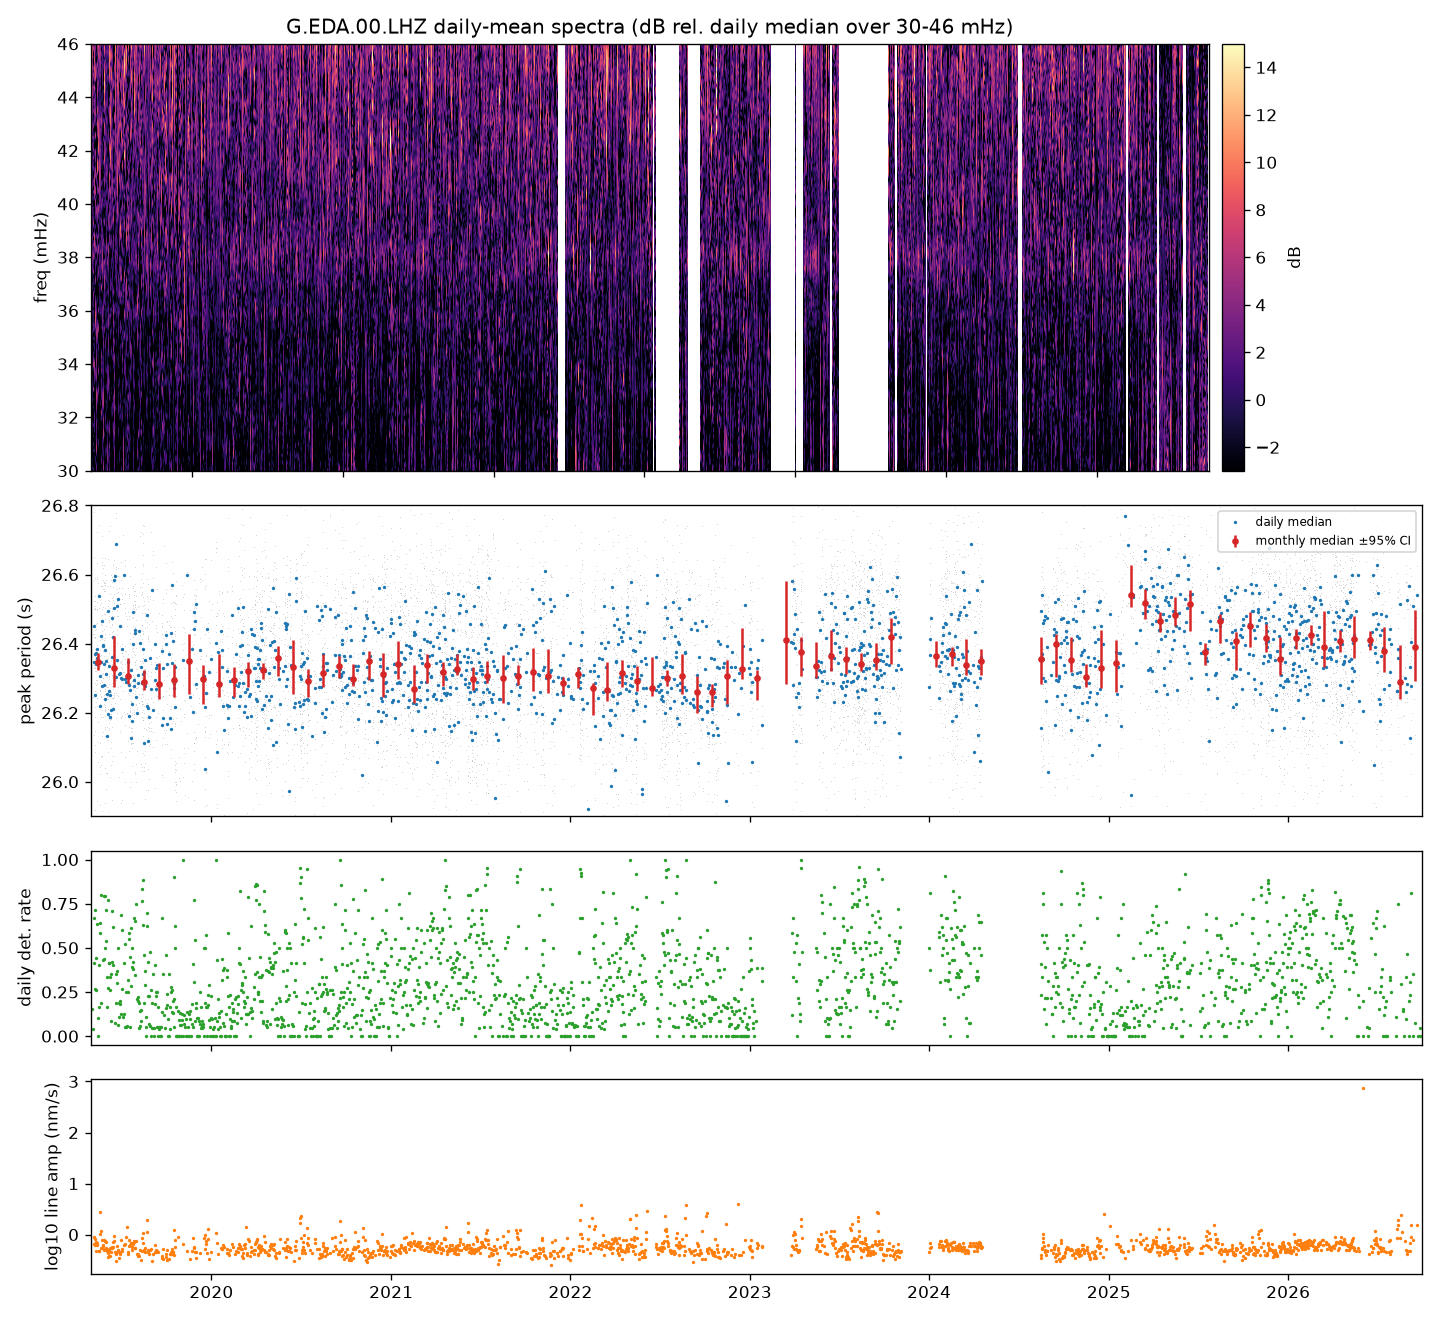
\includegraphics[width=0.9\textwidth]{figs/SI_fig2_longterm_spectra_period.png}
\caption{G.EDA 2019--2026. From top: daily-mean spectra (dB relative to the daily median over 30--46 mHz); peak period of detections (daily and monthly medians with 95\% intervals); daily detection rate; daily line amplitude.}
\label{fig:long}\end{figure}

\begin{figure}[p]\centering
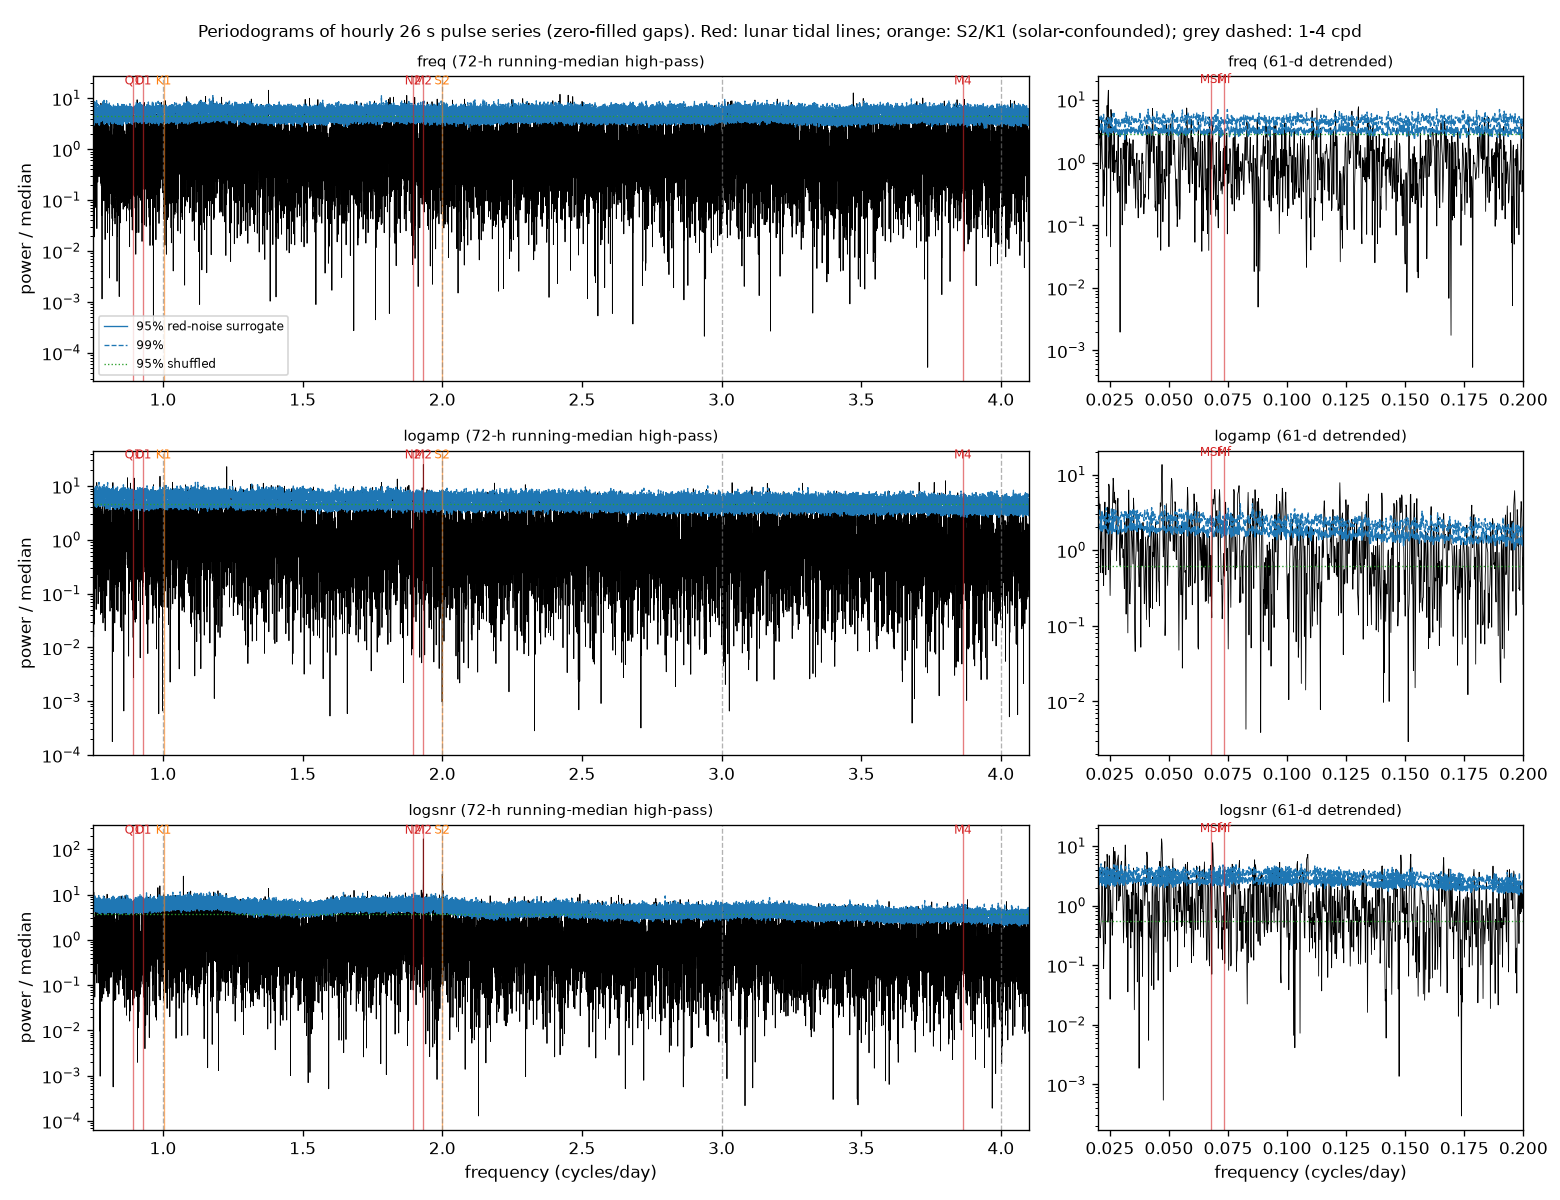
\includegraphics[width=\textwidth]{figs/SI_fig3a_periodogram_fullband.png}
\caption{Periodograms of hourly EDA series (peak frequency, log amplitude, log SNR; gaps zero-filled), 72-h running-median high-passed (left) and 61-day detrended (right), with 95\% and 99\% smoothed-spectrum (red-noise) surrogate levels and 95\% shuffled levels. Red: lunar tidal lines; orange: S2/K1 (solar-confounded).}
\label{fig:pgram}\end{figure}

\begin{figure}[p]\centering
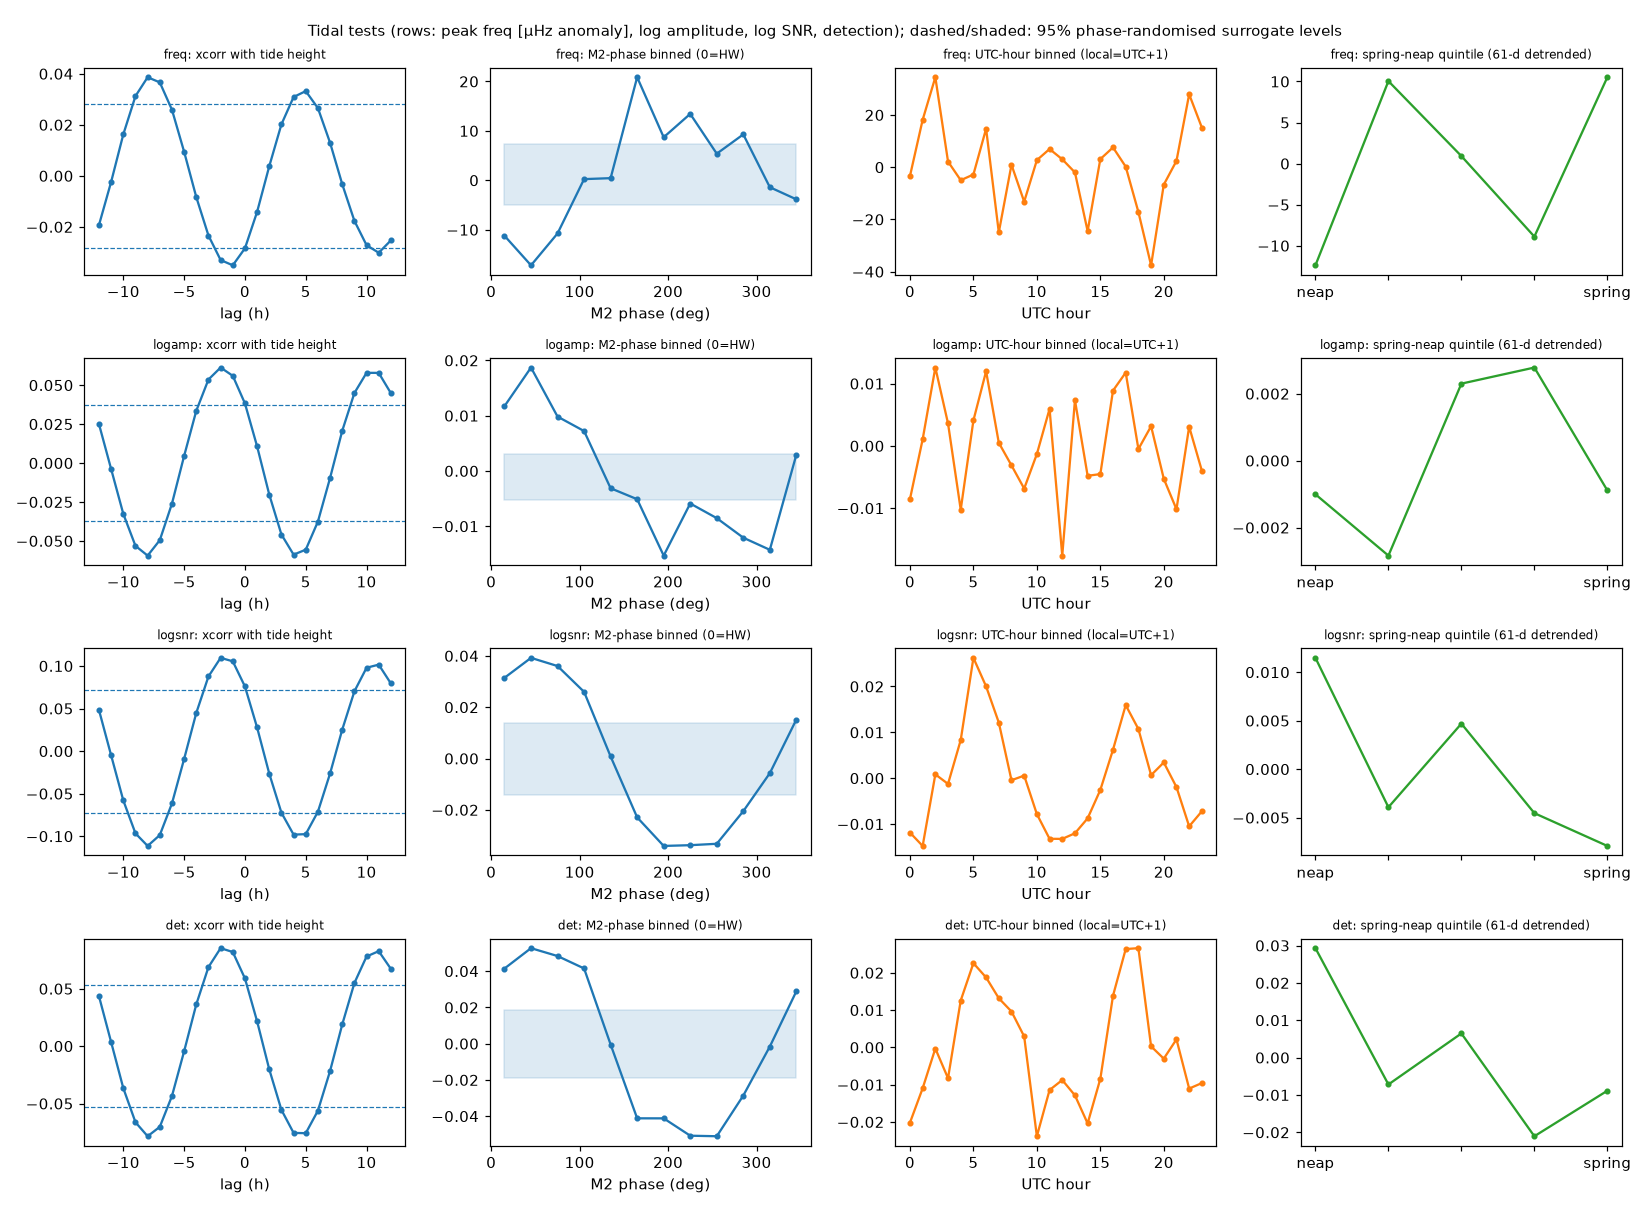
\includegraphics[width=\textwidth]{figs/SI_fig4_tide_binned_xcorr.png}
\caption{Tidal tests at EDA for (rows) peak-frequency anomaly, log amplitude, log SNR and detection. Columns: cross-correlation with tidal height (dashed: 95\% phase-randomised level); binning by M2 phase (shaded: 95\% surrogate range); binning by UTC hour (diurnal/solar control); mean level in spring--neap quintiles of 61-day-detrended series (shown for completeness, no surrogate levels; this is a mean level, not the modulation amplitude).}
\label{fig:xcorr}\end{figure}

\begin{figure}[p]\centering
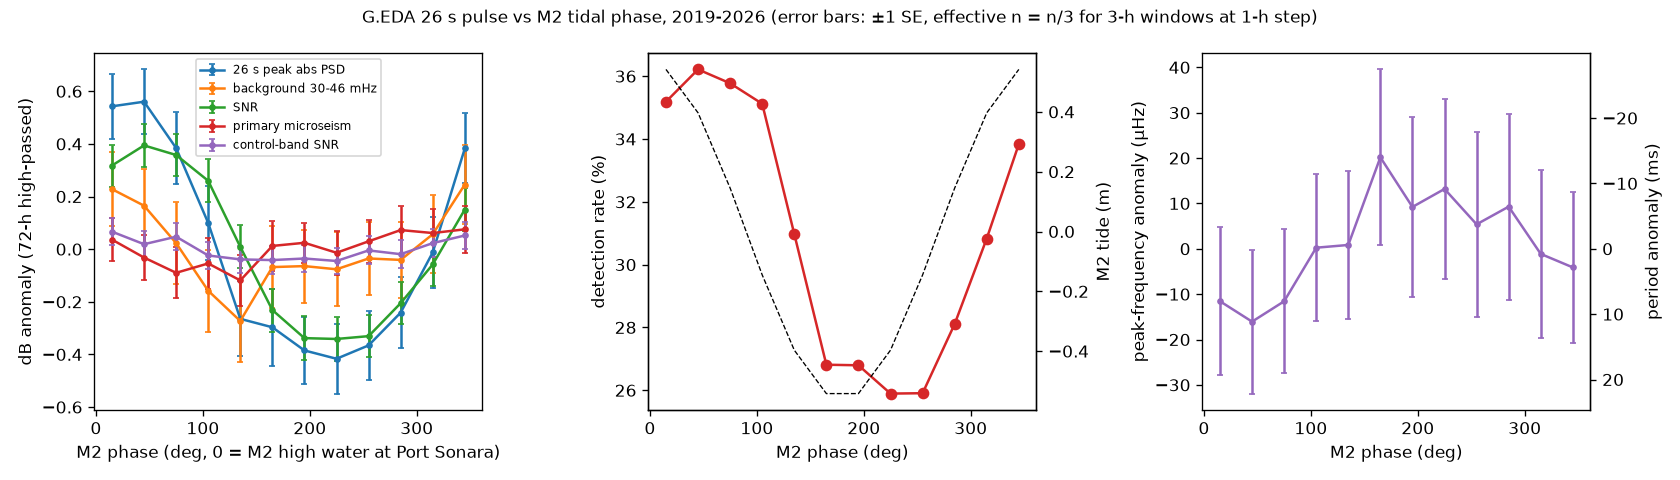
\includegraphics[width=\textwidth]{figs/SI_fig5_M2_phase_controls.png}
\caption{EDA 2019--2026 binned by M2 phase ($\pm1$ SE, effective $n=n/3$). Left: peak PSD, background (30--46 mHz), SNR, primary microseism and control-band SNR. Middle: detection rate with the M2 tide (dashed). Right: peak-frequency anomaly (Text S6).}
\label{fig:ctrl}\end{figure}

\begin{figure}[p]\centering
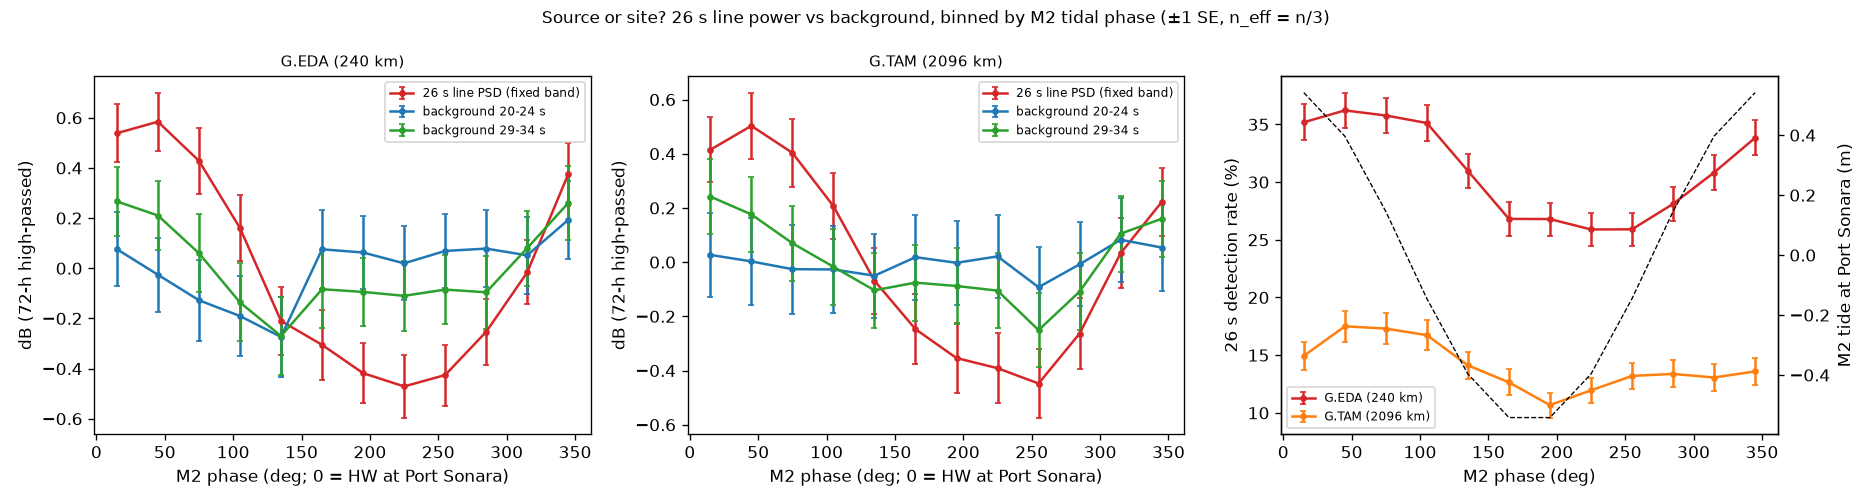
\includegraphics[width=\textwidth]{figs/SI_fig6_source_vs_site.png}
\caption{Line versus background power binned by M2 phase at EDA and TAM (fixed-band line PSD; 20--24 s and 29--34 s backgrounds; $\pm1$ SE), and detection rate at both stations with the tide (dashed).}
\label{fig:svs}\end{figure}

\begin{figure}[p]\centering
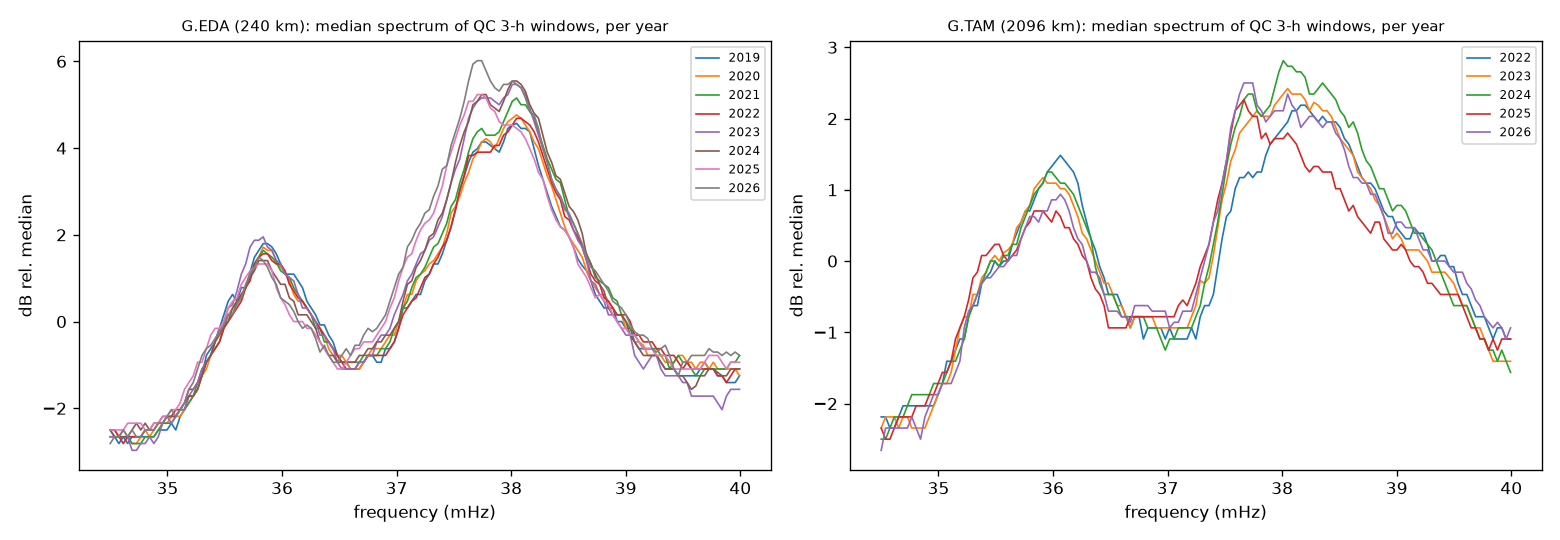
\includegraphics[width=\textwidth]{figs/SI_fig7_yearly_stacks.png}
\caption{Median spectra of quality-controlled 3-h windows per year at EDA (left) and TAM (right), showing the 28 s line near 35.8 mHz and the 26 s doublet near 37.7 and 38.0 mHz, with the change in dominant component in 2025 (Text S7).}
\label{fig:stacks}\end{figure}

\begin{figure}[p]\centering
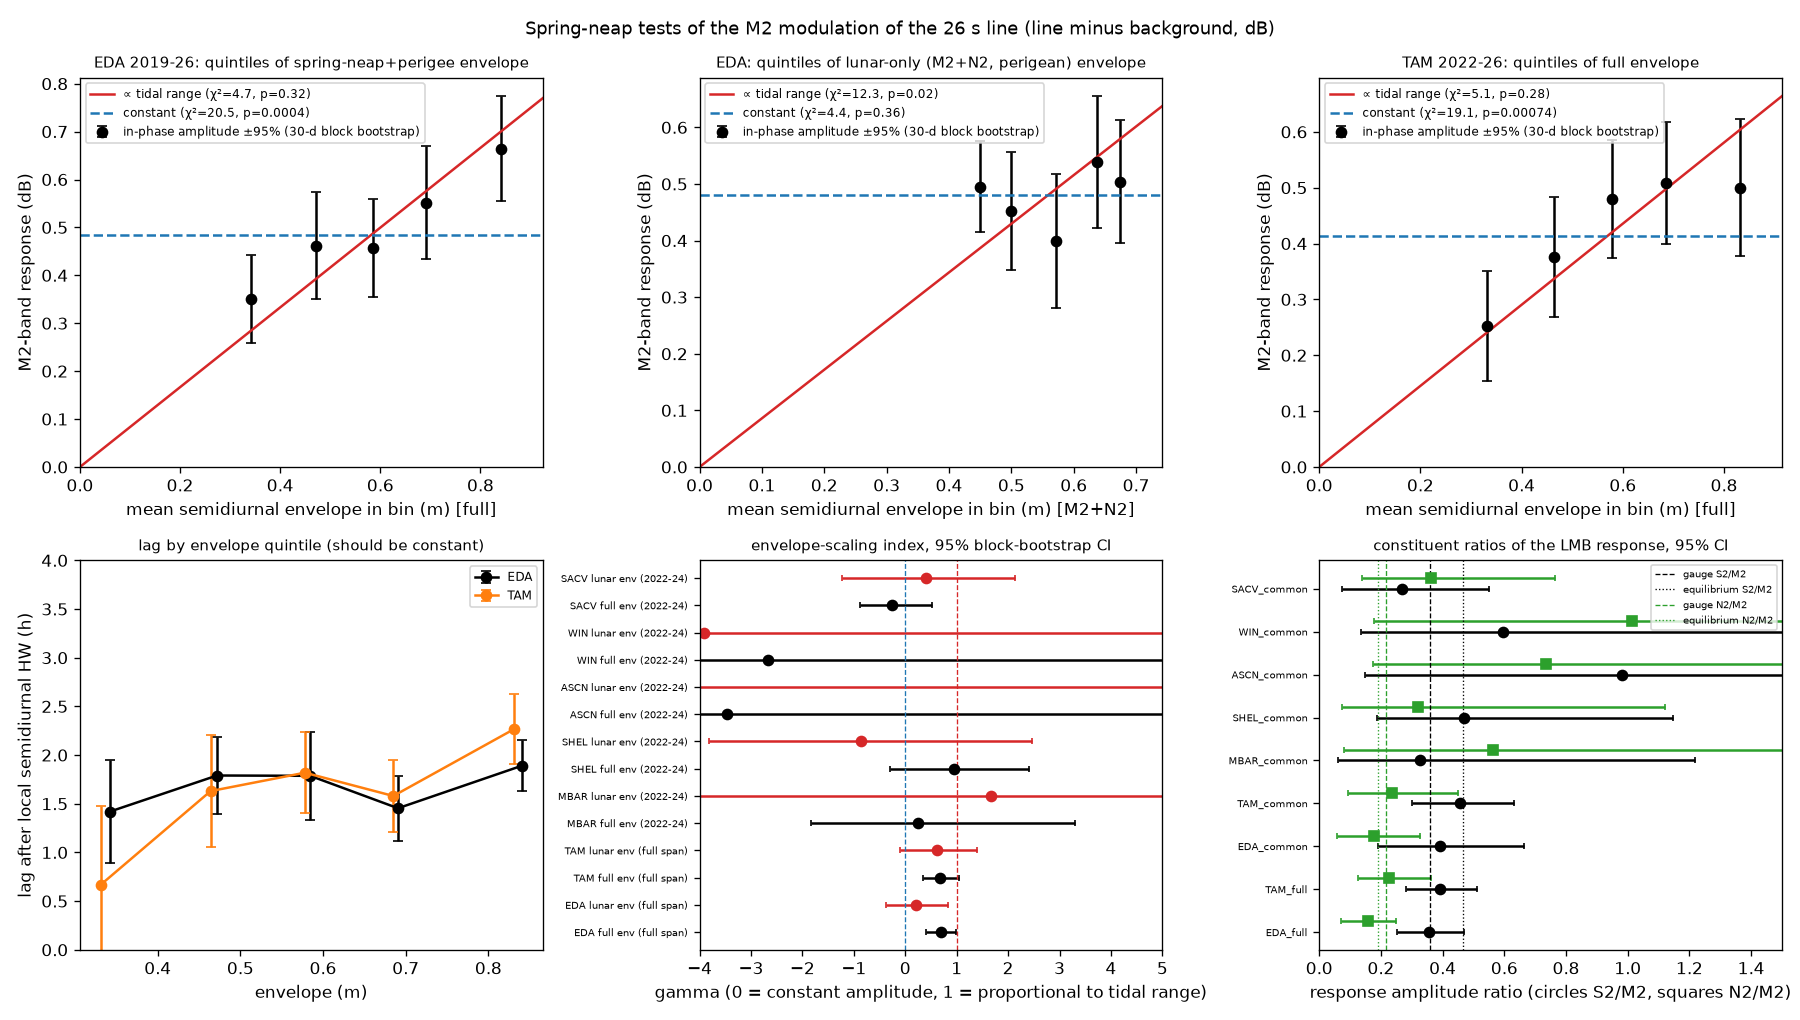
\includegraphics[width=\textwidth]{figs/SI_fig10_springneap.png}
\caption{Spring--neap tests (LMB). Top: in-phase M2-band response in envelope quintiles for EDA (full envelope), EDA (lunar-only M2+N2 envelope) and TAM (full envelope), with proportional (red) and constant (blue) fits. Bottom: lag by envelope quintile; scaling index $\gamma$ for each station with the full and lunar envelopes (note: the lunar envelope in this panel is the incomplete M2+N2 envelope; see Text S5 for the rebuilt envelope); S2/M2 and N2/M2 response ratios compared with the gauge and equilibrium ratios.}
\label{fig:sn}\end{figure}

\begin{figure}[p]\centering
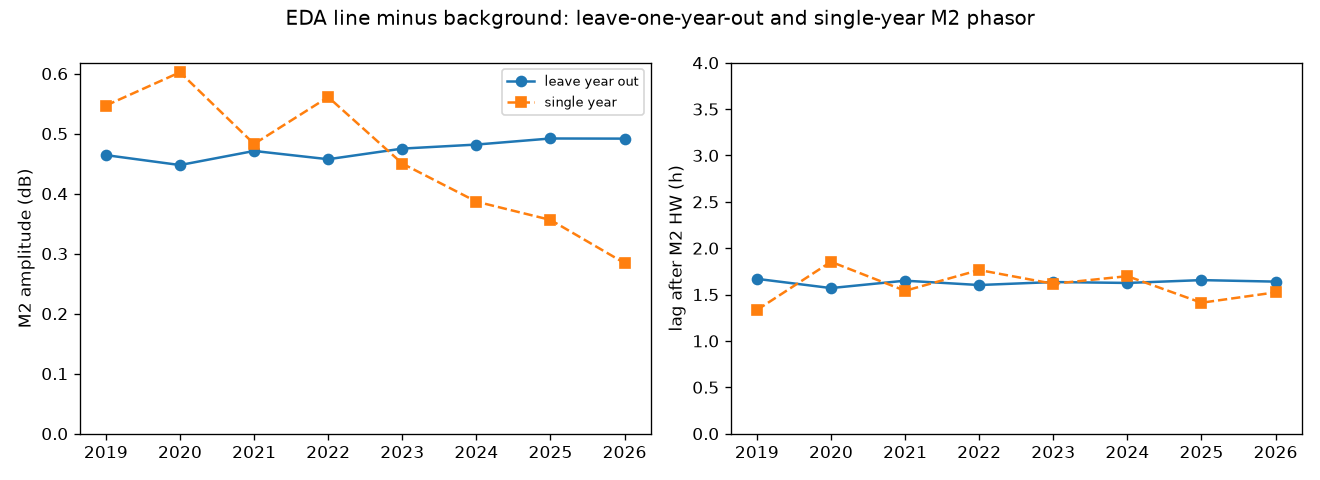
\includegraphics[width=\textwidth]{figs/SI_fig11_loyo.png}
\caption{EDA LMB M2 amplitude (left) and lag (right) leaving out one calendar year (circles) and for single years (squares).}
\label{fig:loyo}\end{figure}

\begin{figure}[p]\centering
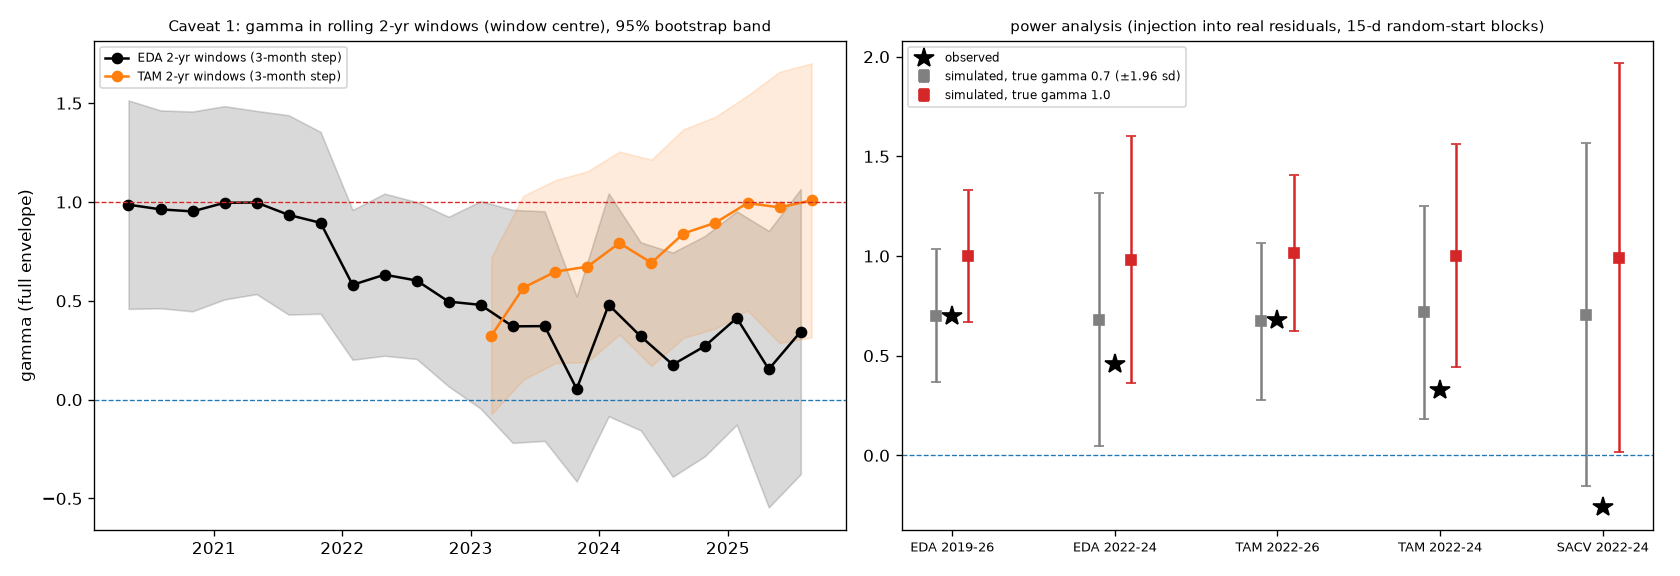
\includegraphics[width=\textwidth]{figs/SI_fig12_caveat1_power_rolling.png}
\caption{Left: $\gamma$ in rolling 2-yr windows (3-month step) at EDA and TAM with 95\% bootstrap bands. Right: power analysis by injection into the real residuals (15-day random-start blocks) for true $\gamma=0.7$ and 1.0, with the observed values (stars).}
\label{fig:cav1}\end{figure}

\begin{figure}[p]\centering
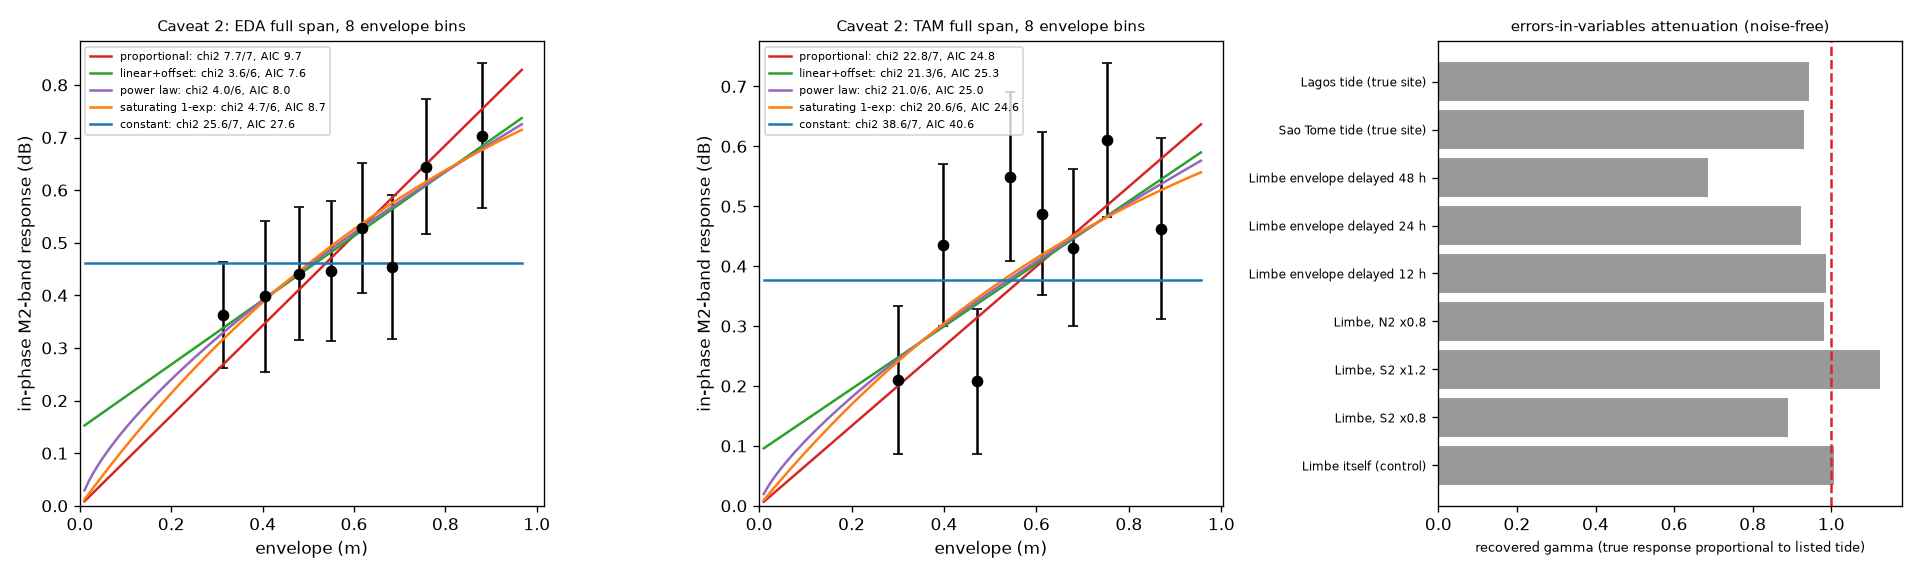
\includegraphics[width=\textwidth]{figs/SI_fig13_caveat2_shapes_eiv.png}
\caption{Left and middle: in-phase response in eight envelope bins (full span) at EDA and TAM with proportional, linear-plus-offset, power-law, saturating and constant fits. Right: recovered $\gamma$ for a noise-free response proportional to alternative tide envelopes (errors-in-variables attenuation).}
\label{fig:cav2}\end{figure}

\begin{figure}[p]\centering
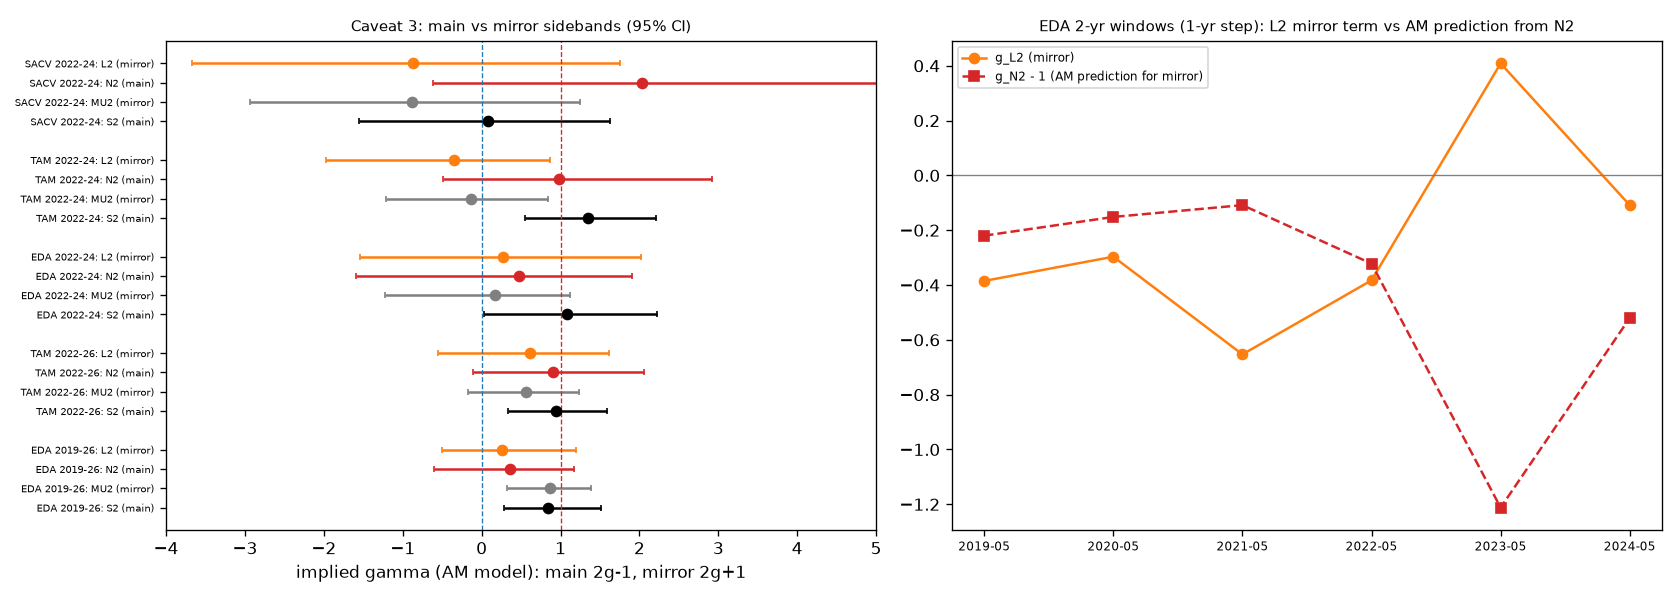
\includegraphics[width=\textwidth]{figs/SI_fig14_caveat3_sidebands.png}
\caption{Left: $\gamma$ implied by main (S2, N2) and mirror (MU2, L2) sidebands under the amplitude-modulation model, by station and period. Right: EDA 2-yr windows (1-yr step), L2 mirror term compared with its AM prediction from N2.}
\label{fig:cav3}\end{figure}

\bibliographystyle{plainnat}
\bibliography{refs}
\end{document}
